\subsection{Xây dựng giả thuyết}
Thông thường, để có thể xây dựng được các giả thuyết nghiên cứu một cách chặt chẽ, ta cần tìm hiểu tổng quan lí thuyết liên quan và từ đó tổng hợp, đề xuất các giả thuyết dựa trên nền tảng lí thuyết đã có. Tuy nhiên, trong phạm vi bài tập này, vì hạn chế trong kiến thức chuyên ngành trong lĩnh vực quản trị lao động, nhóm thực hiện phân tích tỉ lệ sử dụng mạng xã hội (Snapchat, Instagram) theo từng nhóm tình trạng việc làm để có thể đưa ra giả thuyết ban đầu về mối quan hệ giữa việc sử dụng mạng xã hội và tình trạng việc làm của một cá nhân. Hình \ref{fig:using_social_media} dưới đây thể hiện tỉ lệ sử dụng tối thiểu một mạng xã hội (Snapchat, Instgram) của 08 nhóm tương ứng với 08 loại tình trạng việc làm. Đường màu đỏ thể hiện tỉ lệ sử dụng trung bình của toàn thể 08 nhóm nêu trên (18\%).

\begin{figure}[h!]
    \centering
    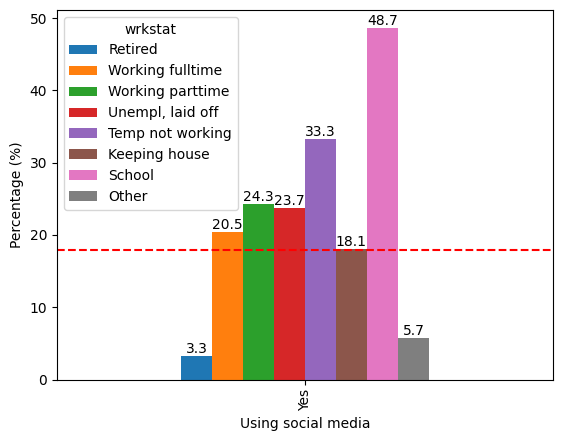
\includegraphics[width=0.6\textwidth]{figures/using_social_media.png}
    \caption{Tỉ lệ sử dụng mạng xã hội của các nhóm tình trạng việc làm}
    \label{fig:using_social_media}
\end{figure}

Từ biểu đồ trên, một cách trực quan có thể thấy tỉ lệ sử dụng mạng xã hội giữa các nhóm tình trạng việc làm có sự khác biệt đáng kể. Cụ thể, nhóm người đã nghỉ hưu (Retired) và nhóm tình trạng khác (Other) có xu hướng ít sử dụng mạng xã hội hơn hẳn so với mặt bằng chung và so với các nhóm còn lại. Ngược lại, nhóm người đang đi học (School) và nhóm tạm thời đang nghỉ việc (Temp not working) lại có xu hướng sử dụng mạng xã hội cao hơn nhiều so với các nhóm khác. Từ phân tích trên, nhóm đề xuất hai (02) giả thuyết như sau:

\textbf{Giả thuyết 1: “Việc sử dụng mạng xã hội và tình trạng việc làm của một cá nhân có mối quan hệ với nhau”}

\textbf{Giả thuyết 2: “Việc sử dụng mạng xã hội có ảnh hưởng đối với tình trạng việc làm của một cá nhân”}

\subsection{Phương pháp kiểm định giả thuyết}
Để kiểm chứng \textbf{Giả thuyết 1}, ta thực hiện kiểm định chi-squared để kiểm tra tính độc lập giữa yếu tố sử dụng mạng xã hội và tình trạng việc làm của một cá nhân. Việc lựa chọn kiểm định chi-squared là phù hợp trong trường hợp này vì ta có thể thỏa mãn được những giả định (assumptions) của chi-squared test, bao gồm: 
\begin{itemize}
    \item Các biến được sử dụng trong phân tích là biến phân loại (biến định danh hoặc có thứ bậc).
    \item Tính độc lập của các quan sát: vì tập dữ liệu được lấy từ nghiên cứu thực nghiệm được thiết kế và triển khai chặt chẽ theo các tiêu chuẩn khoa học, ta có thể giả định rằng tính độc lập của các quan sát thu được thỏa mãn (tức là các quan sát trong tập dữ liệu độc lập với nhau).
    \item Kích thước mẫu đảm bảo mỗi ô trong bảng contingency (Bảng \ref{tab:contingency_table}) đều đạt ngưỡng tối thiểu $(\geq 5)$. Đặc biệt, có nhiều ô trong bảng contingency có kích thước lớn hơn nhiều so với ngưỡng tối thiểu cần thiết, có thể đảm bảo cho kết quả Chi-squared test chính xác hơn.
\end{itemize}

\begin{table}[h!]
    \centering
    \resizebox{\columnwidth}{!}{
        \begin{tabular}{|c|r|r|r|r|r|r|r|r|}
        \hline
        $\begin{array}{c}\text {Using} \\ \text {social media}\end{array}$ & $\begin{array}{r}\text {Keeping} \\ \text {house}\end{array}$ & $\begin{array}{r}\text {Other}\end{array}$ & $\begin{array}{r}\text {Retired}\end{array}$ & $\begin{array}{r}\text {School}\end{array}$ & $\begin{array}{r}\text {Temp not} \\ \text {working}\end{array}$ & $\begin{array}{r}\text {Unempl,} \\ \text {laid off}\end{array}$ & $\begin{array}{r}\text {Working} \\ \text {fulltime}\end{array}$ & $\begin{array}{r}\text {Working} \\ \text {parttime}\end{array}$ \\
        \hline
        No & 74 & 20 & 143 & 18 & 20 & 31 & 439 & 112 \\
        \hline
        Unknown & 157 & 62 & 411 & 21 & 18 & 59 & 611 & 149 \\
        \hline
        Yes & 51 & 5 & 19 & 37 & 19 & 28 & 270 & 84 \\
        \hline
        \end{tabular}
    }
    \caption{Bảng contingency}
    \label{tab:contingency_table}
\end{table}

Liên quan đến \textbf{Giả thuyết 2}, ta xây dựng mô hình hồi quy multinomial logistic để phân loại tình trạng việc làm dựa trên các thông tin trong tập dữ liệu đã cho sau khi đã thực hiện mã hóa (one-hot-encoding), trong đó có bao gồm biến độc lập liên quan đến hành vi sử dụng mạng xã hội của các cá nhân đó. Tiếp theo, việc kiểm định giả thuyết 2 được đưa về bài toán kiểm định tính khác 0 của các hệ số tương ứng với biến độc lập về hành vi sử dụng mạng xã hội (Chi tiết được thể hiện trong tiểu mục tiếp theo). 

\subsection{Kết quả kiểm định giả thuyết}
\subsubsection{Kiểm định tính độc lập giữa việc sử dụng mạng xã hội và tình trạng việc làm của một cá nhân}
$$
\left\{\begin{array}{l}
H_{0}: \text{Việc sử dụng mạng xã hội và tình trạng việc làm của một cá nhân là độc lập với nhau}\\
H_{1}: \text{Việc sử dụng mạng xã hội và tình trạng việc làm của một cá nhân có quan hệ với nhau}
\end{array}\right.
$$

Ta có:
$$
\chi^{2}=\sum \frac{\left(O_{i j}-E_{i j}\right)^{2}}{E_{i j}}
$$

Với:
\begin{itemize}
    \item $O_{i j}$ là tần suất quan sát được của ô $(i, j)$ trong bảng contingency
    \item $E_{i j}$ là tuần suất kì vọng tương ứng với ô $(i, j)$ trong bảng contingency
\end{itemize}

Từ bảng contingency, ta tính được trị số thống kê chi-square là $229.310(df=14)$ với p-value tương ứng là $5.347 * 10^{-41}(\ll 0.05)$. Vì vậy, với mức ý nghĩa $5 \%$, ta bác bỏ giả thiết $H_{0}$, chấp nhận $H_{1}$. Tức là, với độ tin cậy 95\%, ta có thể khẳng định việc sử dụng mạng xã hội và tình trạng việc làm có mối quan hệ với nhau.

\subsubsection{Kiểm định ảnh hưởng của việc sử dụng mạng xã hội đối với tình trạng việc làm của một cá nhân}
Như đã phân tích ở các phần trên, trường dữ liệu email\_total có tỉ lệ trống (null) lớn, vì vậy ta phân chia tập dữ liệu ban đầu thành 02 tập nhỏ hơn: (1) tập dữ liệu gồm các quan sát không bị trống email\_total – Nhóm A, (2) tập dữ liệu gồm các quan sát bị trống giá trị email\_total – Nhóm B.

\textbf{Xét nhóm quan sát A}

Ta có:


Với $x \in\{$'Retired', 'Working fulltime', 'Working parttime', 'Unempl, laid off', 'Temp not working', 'Keeping house', 'School', 'Other'\}

Bài toán kiểm định 1:
$$
\left\{\begin{array}{l}
H_{0}: \beta_{18}=0 \\
H_{1}: \beta_{18} \neq 0
\end{array}\right.
$$

Bài toán kiểm định 2
$$
\left\{\begin{array}{l}
H_{0}: \beta_{19}=0 \\
H_{1}: \beta_{19} \neq 0
\end{array}\right.
$$

Kết quả ước lượng thu được từ tập dữ liệu đã cho được thể hiện trong hình \ref{fig:beta1819}:

\begin{figure}[h!]
    \centering
    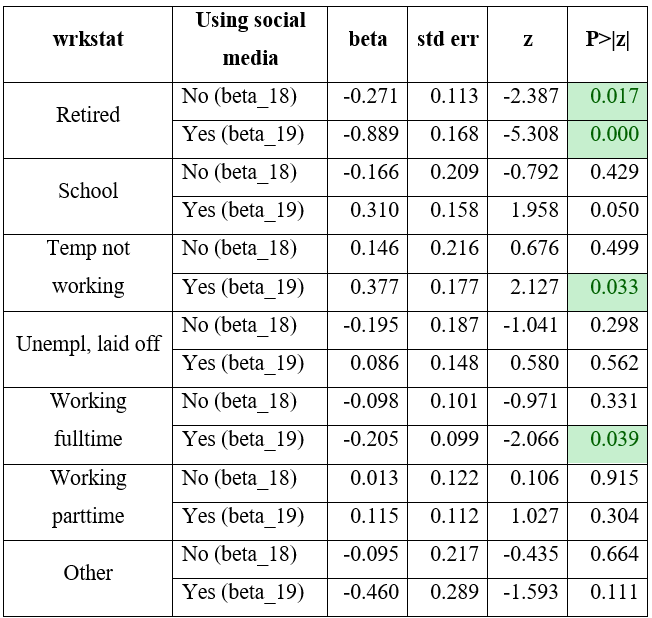
\includegraphics[width=0.6\textwidth]{figures/beta1819.png}
    \caption{Kết quả ước lượng tham số $\beta_{18}, \beta_{19}$ mô hình hồi quy multinomial logistic đối với Nhóm A}
    \label{fig:beta1819}
\end{figure}

Từ kết quả trên, với mức ý nghĩa $5 \%$ ta có thể bác bỏ $H_{0}$ trong một số trường hợp (Retired đối với $\beta_{18}$ và $\beta_{19}$, Temp not working và Working fulltime đối với $\beta_{19}$) và chấp nhận $H_{0}$ trong các trường hợp còn lại. Nhìn chung, từ kết quả này có thể thấy, việc sử dụng mạng xã hội có ảnh hưởng đến tình trạng việc làm của một số cá nhân, tuy nhiên ảnh hưởng này không tồn tại trong mọi trường hợp mà chỉ tồn tại với một số nhóm đối tượng nhất định.


\textbf{Xét nhóm quan sát B}

Ta có:


Với $x \in\{$'Retired', 'Working fulltime', 'Working parttime', 'Unempl, laid off', 'Temp not working', 'Keeping house', 'School', 'Other'\}

Bài toán kiểm định 1:
$$
\left\{\begin{array}{l}
H_{0}: \beta_{17}=0 \\
H_{1}: \beta_{17} \neq 0
\end{array}\right.
$$
Bài toán kiểm định 2:
$$
\left\{\begin{array}{l}
H_{0}: \beta_{18}=0 \\
H_{1}: \beta_{18} \neq 0
\end{array}\right.
$$

Kết quả ước lượng thu được từ tập dữ liệu đã cho được thể hiện trong hình \ref{fig:beta1718}:

\begin{figure}[h!]
    \centering
    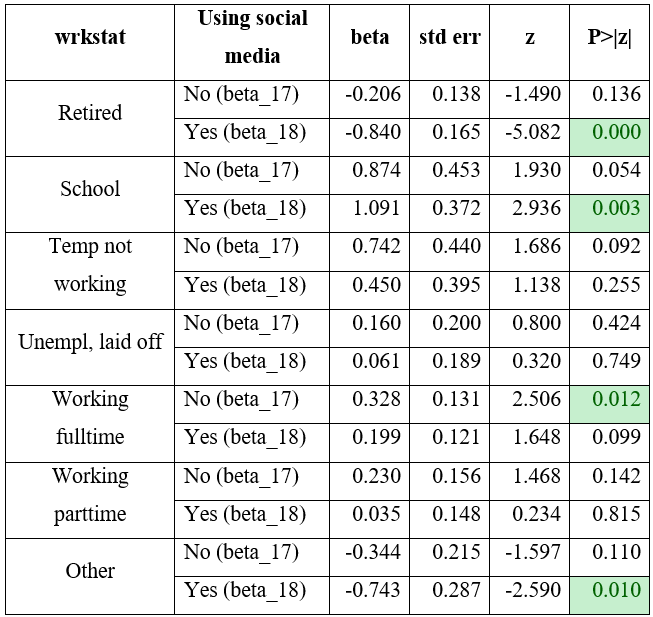
\includegraphics[width=0.6\textwidth]{figures/beta1718.png}
    \caption{Kết quả ước lượng tham số $\beta_{17}, \beta_{18}$ mô hình hồi quy multinomial logistic đối với Nhóm B}
    \label{fig:beta1718}
\end{figure}

Tương tự như trường hợp của nhóm $\mathrm{A}$, đối với các quan sát trong nhóm $\mathrm{B}$, việc sử dụng mạng xã hội có ảnh hưởng đến tình trạng việc làm của một số cá nhân, tuy nhiên ảnh hưởng này cũng không tồn tại trong mọi trường hợp mà chỉ tồn tại với một số nhóm đối tượng nhất định.


\textbf{Kết luận chung}: Bằng các kiểm định thống kê, với mức ý nghĩa $5 \%$, ta có thể khẳng định tồn tại mối quan hệ giữa việc sử dụng mạng xã hội (Snapchat, Instagram) và tình trạng việc làm của một cá nhân. Ảnh hưởng của việc sử dụng mạng xã hội đối với tình trạng việc làm của một cá nhân có ý nghĩa thống kê trong một số trường hợp cụ thể, đặc biệt là đối với nhóm người đang đi học, đang làm việc fulltime hoặc đã nghỉ hưu.